\documentclass[conference]{IEEEtran}
\IEEEoverridecommandlockouts
% The preceding line is only needed to identify funding in the first footnote. If that is unneeded, please comment it out.
\usepackage{cite}
\usepackage{amsmath,amssymb,amsfonts}
\usepackage{algorithmic}
\usepackage{graphicx}
\usepackage{textcomp}
\usepackage{xcolor}
\def\BibTeX{{\rm B\kern-.05em{\sc i\kern-.025em b}\kern-.08em
    T\kern-.1667em\lower.7ex\hbox{E}\kern-.125emX}}
\begin{document}

\title{Efficient categorization of white blood cells by utilizing ResNet50V2 in the
4B-AdditionNet-based CNN network and ant colony optimization workflow\\
{\footnotesize \textsuperscript{*}Note: This paper is the result of a research practice course handout, the results are made up}
}

\author{\IEEEauthorblockN{1\textsuperscript{th} Bustya Balázs}
\IEEEauthorblockA{\textit{Eötvös Loránd University} \\
\textit{Faculty of Informatics}\\
Budapest, Hungary}
\and
\IEEEauthorblockN{2\textsuperscript{th} Csizmadia Árpád}
\IEEEauthorblockA{\textit{Eötvös Loránd University} \\
\textit{Faculty of Informatics}\\
Budapest, Hungary}
\and
\IEEEauthorblockN{3\textsuperscript{th} Nagy Norbert Botond}
\IEEEauthorblockA{\textit{Eötvös Loránd University} \\
\textit{Faculty of Informatics}\\
Budapest, Hungary}
\and
\IEEEauthorblockN{4\textsuperscript{th} Novák-Schwartz József}
\IEEEauthorblockA{\textit{Eötvös Loránd University)} \\
\textit{Faculty of Informatics}\\
Budapest, Hungary}
}

\maketitle

\begin{abstract}
The most logical healthcare method is prevention. Analyzing blood samples is an efficient way to discover serious health issues at early stage. 
Based on the count and the distribution of different types of white blood cells (WBC) early diagnosis of severe diseases, like leukemia and others, can be established. 
But process of manual blood sample analysis is very time consuming and costly. To solve this problem researchers have started to build automatic WBC counting and classification 
systems by using machine learning and deep learning technics. Image classification has developed significantly after appearing modern convolutional neural network (CNN) architectures. 
Researchers have achieved better and better results, but there is still room to improve the accuracy and especially the efficiency of the existing models. 
In this research the proposed system, includes the following methodologies: contrast limited adaptive histogram equalization (CLAHE) for preprocessing, 
combination of three networks, namely EfficientNetB0, 4B-AdditionNet and ResNet50V2 for feature extraction, ant colony optimization (ACO) for feature selection and multiple classifiers 
for classification of the WBS images.The chosen dataset is the Blood Cell Images, which is the augmented version of the BCCD  available dataset. The achieved results show nearly the same accuracy, as other state of the art systems, but reduced the run time with one order of magnitude.

\end{abstract}

\begin{IEEEkeywords}
White blood cells · CNN · Classification · Blood Cell Images dataset · Feature extraction · ResNet50V2
\end{IEEEkeywords}

\section{Introduction}
This document is a model and instructions for \LaTeX.
Please observe the conference page limits. 



The amount of blood in the human body can depend on a few factors, like your sex, how much you weigh, and even where you live, but generally equivalent to 7\% of the body weight. The amount of blood in the human body differs based on where you live. For example, people who live at higher altitudes usually have more blood because there isn’t as much oxygen at lower altitudes. The main component of the blood is plasma, which takes up 55\% of it.
The plasma allows the blood to flow freely throughout the entire body inside blood vessels. Based on different attributes of the blood’s cellular components, like colour, size, texture, composition and shape, they are separated into three cell types: erythrocytes also known as Red Blood Cells (RBC), leukocytes (White Blood Cells) and thrombocytes. Observing these molecules under the microscope, they have distinct shapes and sizes, WBCs being the larger ones due to the presence of nuclei and cytoplasm inside them. 
Based on these features WBC are further divided into two types: granulocytes and agranulocytes. 
Granulocytes are the most common WBC types defined by the granules inside their cytoplasm. The granulocytes, if dyed, can be categorized into four subtypes. These types differ in the colour of the granule stains inside the cytoplasm. The four cell types are neutrophils, eosinophils, basophils, and mast cells. The other type of WBC are agranulocytes that don't have granules in their cytoplasm and are further categorized into lymphocytes and monocytes.

%figure about WBC cells

A sample of 1 µl of human blood sample contains between 4000 and 11000 WBC. The distribution of different WBC types are the followings: neutrophils between 40\% and 70\%, lymphocytes between 20\% and 45\%, monocytes between 2\% and 10\%, eosinophils between 1\% and 6\% and basophils under 1\%. Although basophils make up less than 1\% of the blood, they play an important role in the health of humans. Any minor imbalance can cause serious health issues, e.g., leukemia, 
% https://www.sciencedirect.com/science/article/pii/S0169260718317802?via%3Dihub
which has been considered as the leading death cause among various cancers due to lack of proper treatment. So it is important to diagnose the disease in the early stage. To avoid these kinds of diseases, it is necessary to determine the distribution and the exact count of WBC in the body. At the present there are two commonly used ways to achieve this: the first method involves a specialist who manually counts the cells with the help of a hemocytometer, while the other method is using an automated analyzer.
%https://mural.uv.es/basgaros/Cell-counting-Neubauer-chamber.pdf
%https://www.sciencedirect.com/science/article/pii/B978012427150050098X?via%3Dihub

Complete blood count
%https://www.sciencedirect.com/science/article/pii/S0956566319310139?via%3Dihub
is a blood analyzer which allows one to determine the count of the blood cells present in the body. This allows the diagnosis of various disorders, for example, a lower WBC count than normal, called leukopenia, can forecast the presence of marrow cancer, autoimmune diseases, thyroid disorder, etc. A higher WBC count than normal can be a sign of a foreign substance present in the body. This is called leukocytosis and can cause several serious diseases like leukemia, marrow malformation, etc. In the treatment of these disorders, the key aspect is early diagnosis. In the treatment of leukemia early diagnosis greatly increases the chance of recovery, especially in children.

To achieve an early diagnosis, efficient and fast techniques are necessary so that the count and state of WBC can be determined to conclude results. 


\section{Literature review}
The number of researches of traditional machine learning (TML) and deep learning (DL) for leucocytes classification shows exponential growth in recent times.
%KHAN, Siraj, et al. A review on traditional machine learning and deep learning models for WBCs classification in blood smear images. IEEE Access, 2020, 9: 10657-10673.
DL approaches has the advantage over TML to offer highly automated systems, because in case of DP, feature extraction is learned from data and not designed by humans, as in case of TML.
For this reason DL solutions using CNN got great attention from researchers, especially since modern CNN architectures appeared.

The 
%KHAN, Siraj, et al. A review on traditional machine learning and deep learning models for WBCs classification in blood smear images. IEEE Access, 2020, 9: 10657-10673.
survey collects 
The WBS detection process with CNN is structured from 4 main steps: preprocessing, feature extraction, feature selection and classification.
Our research is based on 
%SHAHZAD, Asim, et al. Categorizing white blood cells by utilizing deep features of proposed 4B-AdditionNet-based CNN network with ant colony optimization. Complex & Intelligent Systems, 2022, 8.4: 3143-3159.


\subsection{}

\color{green} \end
\color{red} \end
\section{Materials and methods}

This part presents the proposed tuning and modification on the 4B-AdditionNet
%https://link.springer.com/article/10.1007/s40747-021-00564-x#Sec3
CNN architecture alongside the description of the main steps of the whole process to classify WBCs. The classification process includes the preprocessing of the blood smear images using CLAHE, the feature extraction using the combination of three networks, namely EfficientNetB0, 4B-AdditionNet and ResNet50V2, the feature selection using ant colony optimization and the classification using multiple classifiers. The steps of the whole process are discussed in the upcoming sections.

\subsection{Image preprocessing}

To enhance the images CLAHE
%https://doi.org/10.21236/ADA014928
is used on the dataset in order to improve the contrast of the smear images and make the cells more prominent. Since CLAHE works with one channel images, the images are splitted into three channels, one for each color channel, and then CLAHE was applied for the separate R, G, B channels. The enhanced images then were merged back together into one final image, which has a much higher contrast compared to the original one.

\subsection{Feature extraction}
%hozzaadott szam - telefonos képek?
In this research, features are extracted from the three different CNNs. These features are extracted from the Blood Cell Images dataset (combined with the images from the mobilephone microscope images.). There are 9957 images from the Blood Cell Images dataset and xxx images from the mobile microscope images. The first network, 4B-AdditionNet extracts 4096 features from its FC-2 layer, while EfficientNetB0 extracts 1000 features from dense|MatMul layer and ResNet50V2 obtains another 1000 features from it's FC1000 layer.


\subsection{Feature selection}

Since there is a large number of different features extracted from CNNs feature selection is used to reduce the dimensionality. A subset of features is selected with a feature optimization algorithm, namely Ant Colony Optimization (ACO). This method is a probabilistic method for choosing optimal paths. It was inspired by the seeking comportment of ants when trying to find a feasible path between the group and the food source. In the beginning, this method was mainly used to try to solve the well-known challenge, the travelling salesman problem. Later it was used for many optimization problems as well.

% table with param values?
ACO has the following parameters:
\begin{itemize}

    \item{the number of ants is m}
    \item{the number of iterations is $t_{max}$}
    \item{the evaporation coefficient is $\rho$ with a value of 0 $\le \rho \le 1$}
    \item{the desirability of graph edges is $\eta$}
    \item{$\alpha \ge 0$, that controls the relative weight of the pheromone}
    \item{$\beta} \ge 0$, that controls the weight of $\eta$
    \item{the amount of initial pheromone concentration is $Q$}

\end{itemize}

In each iteration \emph{t}, every ant \emph{k} begins by randomly selecting a feature. In order to create a subset from the starting feature the ant follows a path. In each step the ant follows the probabilistic transition rule to select the next feature in the path, given by 

P_{ij}^k\left(t\right)=\left\{\begin{array}{l}\frac{\tau_{ij}^\alpha\left(t\right).\eta_{ij}^\beta\left(t\right)}{\sum_{l\in S_i^k}\tau_{il}^\alpha.\eta_{il}^\beta\left(t\right)},\forall j\in S_i^k\\0,\,\,{\text{otherwise}}\end{array}\right.,
where S_{i}^{k} denotes the subset of features that have not been chosen yet, \tau_{ij}(t) represents the pheromone trail between the features i and j, \eta_{ij}(t) represents the heuristic desirability to select feature j when ant k is currently in the feature i.

For each feature subset accuracy is calculated using the formula below:
\mathrm{Accuracy}=\frac{1}{K} \sum\limits_{i=1}^{K}\frac{1}{2}\left({\mathrm{Accuracy}}_{i}^{\mathrm{Train}}+{\mathrm{Accuracy}}_{i}^{\mathrm{Test}}\right),
where K denotes the folds set for the K-fold cross-validation procedure to calculate the subset accuracy.
After calculating the accuracies of the feature subsets, the one with the highest accuracy is chosen and the pheromone trail in the feature space is updated based on this trail.
The same process is repeated for all ants and then finally the subset with the best accuracy is found.

\subsection{Feature fusion}

In the classification process only a single feature vector can be used for classification. To create a single feature vector multiple feature vectors are concatenated horizontally. The purpose of using a single feature vector is to possibly help with the reduction of the error rate. To conduct all five experiments on the designed network, feature fusion is used to create multiple feature vectors with different combinations of features. The features from the three CNNs have been fused serially: the first features are from 4B-AdditionNet, the middle ones are extracted from EfficientNetB0 and the last ones are extracted from ResNet50V2.

\subsection{Classification}

The last step is classification. This is the process of predicting a class label for a given image. Different classifiers such as SVM,
%https://link.springer.com/article/10.1007/BF00994018
LDA,
%https://onlinelibrary.wiley.com/doi/10.1111/j.1469-1809.1936.tb02137.x
and KNN has been used to classify WBC into four categories. The classifiers use fivefold cross-validaiton. The SVMs, namely Linear, Cubic and Quadratic SVM classifiers utilize a Box Constraint of 1 and a Coding Design of OneVsOne. The predictions are measured with multiple performance estimation methods. CSVM is noted to have the highest accuracy while LDA is the fastest one with acceptable accuracy.

\section{Dataset}

The dataset chosen for this study is the Blood Cell Images dataset.
%https://www.kaggle.com/datasets/paultimothymooney/blood-cells
This dataset is the augmented version of the BCCD 
%https://github.com/Shenggan/BCCD_Dataset
dataset. BCCD is a publicly available dataset which divides blood smear images into three classes: RBC, WBC, and Platelets.
The Blood Cell Images dataset contains 12,500 augmented images of blood smears that are divided into four categories: Eosinophil, Lymphocyte, Monocyte, and Neutrophil.
The augmented images have a dimension of 320 x 240 pixels, the bit depth is 24. The images are RGB images, so they have 3 channels and a horizontal and vertical resolution depth of 96 dots per inch (dpi).
%figure about images
\section{Execution environment}
The training process were conducted on a Windows 11 desktop PC with a AMD Ryzen 9 7950X with 16 cores and 32 threads. The CPU was overclocked to a base clock of 4.7 Ghz and we achieved a respectable 5.9 Ghz single core boost performance. The PC had 16GBs of DDR4-4400 RAM, and a CUDA enabled Nvidia GeForce GTX rtx 3090 GPU with 24 GBs of Video RAM (VRAM). Our system consumed 900W of power. The network design, testing, training, and the final experimentation process were performed using the MATLAB R2020b software package.
\section{Results and discussion}

The main objective of this study is to classify WBCs with improved performance while keeping the best possible accuracy while utilizing ResNet50V2 instead of ResNet50 in the classification pipeline discussed earlier (Sec. \ref{methods}) and reducing the number of features needed.
The following subsections contain the outcome and assessment of the performed experiments and they are subsequently explained in detail.

\subsection{Test No. 1 (2100 features)}
For this test we kept the original feature size to compare the result from (papaer1).
This test contains a total of 2100 features with 600 from 4B-AdditionNet, 900 from ResNet50, and 600 from EfficientNetB0. 
The final feature vector after fusion is of size $9957*2100$.
We achieved an Ac of 97.58\% with a Se of 96.56\%, Sp of 98.24\%, Pr of 94.85\%, and an F1 score of 95.69\%, with a runtime of 14.73 s. 
Figure \ref{test1} shows the detailed results for the classifiers, it illustrates the training time and Accuracy for all six classifiers.
Our accuracy is close to the original, but our runtime decreased almost tenfold.

\begin{figure}[htbp]
    \begin{center}
    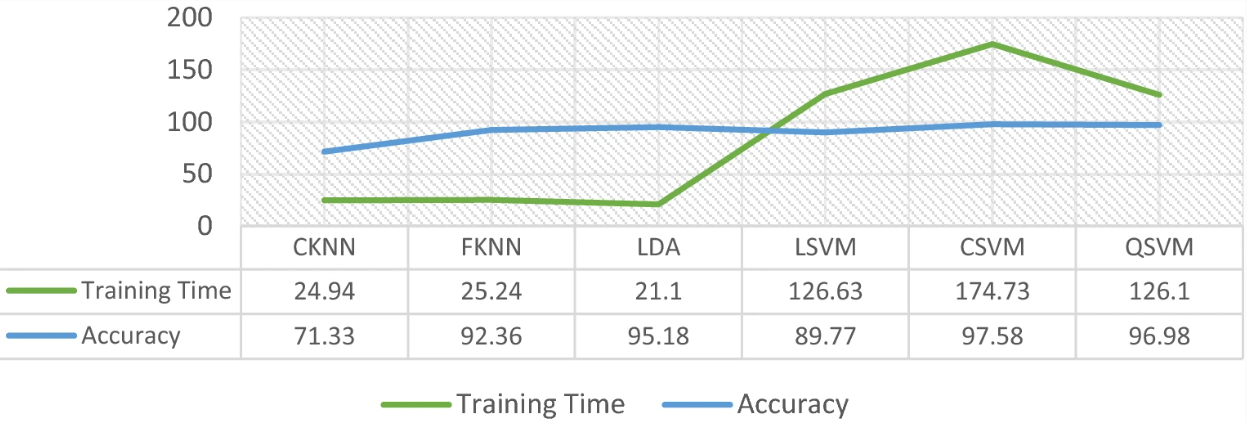
\includegraphics[scale=0.25]{test1.png}
    \end{center}
    \caption{Test No.1 Results}
    \label{test1}
\end{figure}

\subsection{Test No. 2 (1600 features)}

For this test we kept the original feature size to compare the result from (papaer1).
This test contains a total of 1600 features with 500 from 4B-AdditionNet, 700 from ResNet50, and 400 from EfficientNetB0. 
The final feature vector after fusion is of size $9957*1600$.
We achieved an Ac of 96.58\% with a Se of 95.56\%, Sp of 97.24\%, Pr of 93.85\%, and an F1 score of 94.69\%, with a runtime of 13.73 s. 
Figure \ref{test1} shows the detailed results for the classifiers, it illustrates the training time and Accuracy for all six classifiers.
This test contained less features, which resulted in worse accuracy, however we didn't gain too much performance.

\begin{figure}[htbp]
    \begin{center}
    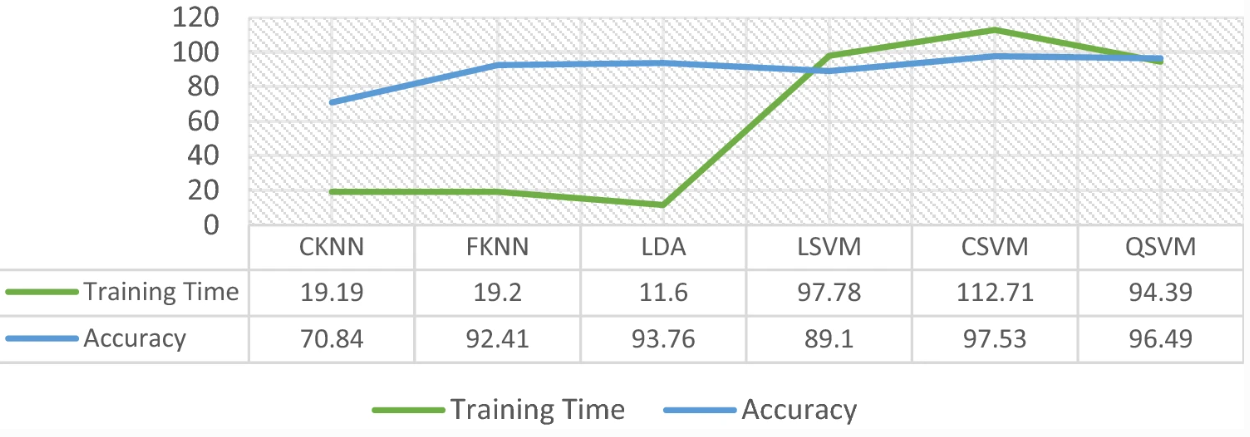
\includegraphics[scale=0.25]{test2.png}
    \end{center}
    \caption{Test No.2 Results}
    \label{test2}
\end{figure}

\subsection{Test No. 3 (1200 features)}

For this test we kept the original feature size to compare the result from (papaer1).
This test contains a total of 1200 features with 400 from 4B-AdditionNet, 400 from ResNet50, and 400 from EfficientNetB0. 
The final feature vector after fusion is of size $9957*1200$.
We achieved an Ac of 95.58\% with a Se of 94.56\%, Sp of 96.24\%, Pr of 92.85\%, and an F1 score of 93.69\%, with a runtime of 12.73 s. 
Figure \ref{test1} shows the detailed results for the classifiers, it illustrates the training time and Accuracy for all six classifiers.
This test contained much less features, which resulted in even worse accuracy, however we didn't gain too much performance.

\begin{figure}[htbp]
    \begin{center}
    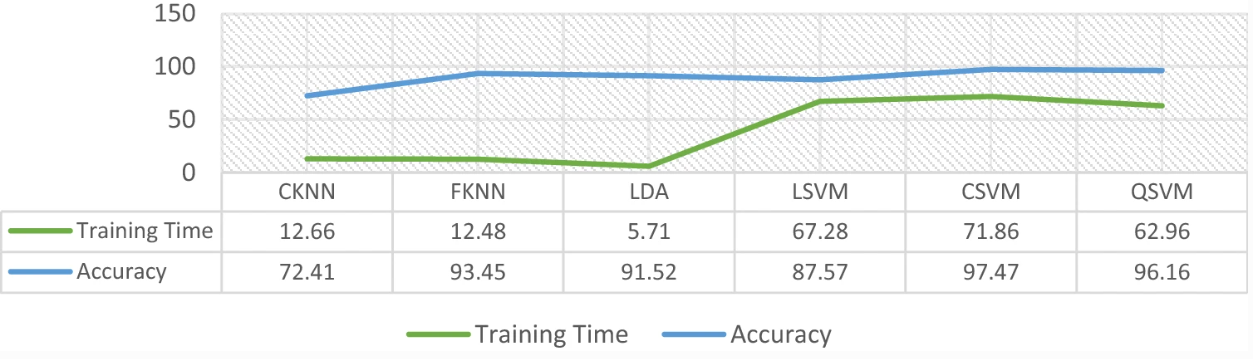
\includegraphics[scale=0.25]{test3.png}
    \end{center}
    \caption{Test No.3 Results}
    \label{test3}
\end{figure}

\section{Conclusion}

We achieved 10 fold runtime decrease with ResNet50V2 using 2100 feature sets while keeping accuracy close to the original.
From the tests No. 2 and No. 3 we conclude that replacing ResNet50 with ResNet50V2 is a good way to decrease runtime while keeping good accuracy, but from the results we observed that the new method is sensitive to low feature sizes.
However for feature reduction we observed a negative result for runtime improvement, meaning that the original feature sizes are also performance optimal in the current pipeline.

\section{Future work}

While existing methods already achieved very high accuracy in blood cell classification, other aspects as speed and generality could be still improved as shown by this study. 
Further advances can be made by including and fusing together bigger Blood Cell Images datasets, like LISC, which would include an other type of cell to classify, which could refine our classification method to perform better across diverse datasets.
Performance can also be further improved by using bigger and more diverse datasets and by reducing the
amount of extracted features.

\section*{Acknowledgment}

We would like to say thank you to our research methodology practice teacher Turcsányi-Szabó Márta and lecturer Dr. Horváth Zoltán, who teached us the paper writing methodology and guided us with good advices.
We are grateful to Eötvös Loránd Tudományegyetem for providing us accessibility to the newest and most prestigious research journals.
This work would not have been possible without the supervision of the bravest and frendliest guard dog Maya, who always encouraged us to work hard.

\begin{figure}[htbp]
    \begin{center}
    
\includegraphics[scale=0.16]{IMG_20221019_165459.jpg}
    \end{center}
    \caption{Maya is our patronus.}
\end{figure}


\section*{Peer review certification}
This paper went through a robust peer review process by anonymous field experts (Fig. \ref{aiProf}).

\begin{figure}[htbp]
    \begin{center}
    
\includegraphics[scale=0.10]{peer_review.png}
    \end{center}
    \caption{Unknown AI professional.}
    \label{aiProf}
\end{figure}

\section*{Declarations}

\textbf{Conflict of interest} On behalf of all authors, the corresponding author
states that there is no conflict of interest.

\begin{thebibliography}{00}
\bibitem{b1} BUSNATU, Ștefan, et al. Clinical Applications of Artificial Intelligence—An Updated Overview. Journal of Clinical Medicine, 2022, 11.8: 2265.
\bibitem{b2} PFEIL, Juliane, et al. Examination of blood samples using deep learning and mobile microscopy. BMC bioinformatics, 2022, 23.1: 1-14.
\bibitem{b3} HUANG, Qian, et al. Blood cell classification based on hyperspectral imaging with modulated Gabor and CNN. IEEE journal of biomedical and health informatics, 2019, 24.1: 160-170.
\bibitem{b4} BOLDÚ, Laura, et al. A deep learning model (ALNet) for the diagnosis of acute leukaemia lineage using peripheral blood cell images. Computer Methods and Programs in Biomedicine, 2021, 202: 105999.
\bibitem{b5} SHAHZAD, Asim, et al. Categorizing white blood cells by utilizing deep features of proposed 4B-AdditionNet-based CNN network with ant colony optimization. Complex and Intelligent Systems, 2022, 8.4: 3143-3159.
\bibitem{b6} RAHIMZADEH, Mohammad; ATTAR, Abolfazl. A modified deep convolutional neural network for detecting COVID-19 and pneumonia from chest X-ray images based on the concatenation of Xception and ResNet50V2. Informatics in medicine unlocked, 2020, 19: 100360.
\bibitem{b7} KHAN, Siraj, et al. A review on traditional machine learning and deep learning models for WBCs classification in blood smear images. IEEE Access, 2020, 9: 10657-10673.
\bibitem{b8} TAVAKOLI, Nasrin, et al. Detection of abnormalities in mammograms using deep features. Journal of Ambient Intelligence and Humanized Computing, 2019, 1-13. 
\bibitem{b9} PRINYAKUPT, Jaroonrut; PLUEMPITIWIRIYAWEJ, Charnchai. Segmentation of white blood cells and comparison of cell morphology by linear and naïve Bayes classifiers. Biomedical engineering online, 2015, 14.1: 1-19. 
\bibitem{b10} JIANG, Kan; LIAO, Qing-Min; XIONG, Yuan. A novel white blood cell segmentation scheme based on feature space clustering. Soft Computing, 2006, 10.1: 12-19.
\bibitem{b11} ZHONG, Zhen, et al. White blood cell segmentation via sparsity and geometry constraints. IEEE Access, 2019, 7: 167593-167604.
\bibitem{b12} PAL, Kuntal Kumar; SUDEEP, K. S. Preprocessing for image classification by convolutional neural networks. In: 2016 IEEE International Conference on Recent Trends in Electronics, Information and Communication Technology (RTEICT). IEEE, 2016. p. 1778-1781.
\bibitem{b13} SALAU, Ayodeji Olalekan; JAIN, Shruti. Feature extraction: a survey of the types, techniques, applications. In: 2019 International Conference on Signal Processing and Communication (ICSC). IEEE, 2019. p. 158-164.
\bibitem{b14} HEGDE, Roopa B., et al. Feature extraction using traditional image processing and convolutional neural network methods to classify white blood cells: a study. Australasian physical & engineering sciences in medicine, 2019, 42.2: 627-638. 
\bibitem{b15} SHARIF, Muhammad, et al. A framework for offline signature verification system: Best features selection approach. Pattern Recognition Letters, 2020, 139: 50-59.
\bibitem{b16} SABA, Tanzila, et al. Categorizing the students’ activities for automated exam proctoring using proposed deep L2-GraftNet CNN network and ASO based feature selection approach. IEEE Access, 2021, 9: 47639-47656.
\bibitem{b17} SHAH, Jamal Hussain, et al. Facial expressions classification and false label reduction using LDA and threefold SVM. Pattern Recognition Letters, 2020, 139: 166-173.
\bibitem{b18} BRIDLE, John S. Probabilistic interpretation of feedforward classification network outputs, with relationships to statistical pattern recognition. In: Neurocomputing. Springer, Berlin, Heidelberg, 1990. p. 227-236.
\bibitem{b19} BANIK, Partha Pratim; SAHA, Rappy; KIM, Ki-Doo. An automatic nucleus segmentation and CNN model based classification method of white blood cell. Expert Systems with Applications, 2020, 149: 113211. 
\bibitem{b20} ALMEZHGHWI, Khaled; SERTE, Sertan. Improved classification of white blood cells with the generative adversarial network and deep convolutional neural network. Computational Intelligence and Neuroscience, 2020, 2020.
\bibitem{b21} TAVAKOLI, Sajad, et al. New segmentation and feature extraction algorithm for classification of white blood cells in peripheral smear images. Scientific Reports, 2021, 11.1: 1-13.
\bibitem{b22} FERREIRA, Carlos A., et al. Classification of breast cancer histology images through transfer learning using a pre-trained inception resnet v2. In: International conference image analysis and recognition. Springer, Cham, 2018. p. 763-770. 
\bibitem{b23} DOMINIC, Nicholas, et al. Transfer learning using inception-ResNet-v2 model to the augmented neuroimages data for autism spectrum disorder classification. Commun. Math. Biol. Neurosci., 2021, 2021: Article ID 39. 
\end{thebibliography}
\vspace{12pt}
\color{red}
\end{document}

